%%%%%%%%%%%%%%%%%%%%%%%%%%%%%%%%%%%%%%%%%%%%%%%%%%%%%%%%%%%%%%%%%%%%%%%%%%%%%%%%
%2345678901234567890123456789012345678901234567890123456789012345678901234567890
%        1         2         3         4         5         6         7         8

\documentclass[letterpaper, 10 pt, conference]{ieeeconf}  % Comment this line out if you need a4paper

%\documentclass[a4paper, 10pt, conference]{ieeeconf}      % Use this line for a4 paper

\IEEEoverridecommandlockouts                              % This command is only needed if 
                                                          % you want to use the \thanks command

\overrideIEEEmargins                                      % Needed to meet printer requirements.

%In case you encounter the following error:
%Error 1010 The PDF file may be corrupt (unable to open PDF file) OR
%Error 1000 An error occurred while parsing a contents stream. Unable to analyze the PDF file.
%This is a known problem with pdfLaTeX conversion filter. The file cannot be opened with acrobat reader
%Please use one of the alternatives below to circumvent this error by uncommenting one or the other
%\pdfobjcompresslevel=0
%\pdfminorversion=4

% See the \addtolength command later in the file to balance the column lengths
% on the last page of the document

% The following packages can be found on http:\\www.ctan.org
\usepackage{graphics} % for pdf, bitmapped graphics files
\usepackage{epsfig} % for postscript graphics files
\usepackage{mathptmx} % assumes new font selection scheme installed
\usepackage{times} % assumes new font selection scheme installed
\usepackage{amsmath} % assumes amsmath package installed
\usepackage{amssymb}  % assumes amsmath package installed
\usepackage{booktabs}
\usepackage{multirow}
\usepackage{xcolor}
\usepackage{threeparttable} % 需要添加在 preamble 中
\usepackage{subcaption}

% 新加的

\title{\LARGE \bf
MESC-DAST: A Unified Framework for Medical Image Classification and Grading
}


\author{Yunxuan Peng$^{1}$, Hongyu Yan$^{1}$, Yingshan Shen$^{1,*}$
    \thanks{This work was not supported by any organization}% <-this % stops a space
    \thanks{*Corresponding author: Yingshan Shen. E-mail: shenyingshan@scnu.edu.cn.}% <-this % stops a space
    \thanks{$^{1}$Yunxuan Peng, Hongyu Yan, Yingshan Shen, Aberdeen Institute of Data Science and Artificial Intelligence, South China Normal University, Foshan, China
        {\tt\small 20223803032@m.scnu.edu.cn, 20223803065@m.scnu.edu.cn}} % <- First and second author<- Corresponding author
}


\begin{document}



\maketitle
\thispagestyle{empty}
\pagestyle{empty}


%%%%%%%%%%%%%%%%%%%%%%%%%%%%%%%%%%%%%%%%%%%%%%%%%%%%%%%%%%%%%%%%%%%%%%%%%%%%%%%%
\begin{abstract}

Medical image classification and grading remain challenging due to low contrast, complex lesion morphology, and pronounced multi-scale structural variations. In addition, ordinal medical grading tasks exhibit structured inter-class relationships that are not well captured by conventional one-hot supervision. To address these issues, we propose a unified framework that combines a Median-enhanced Spatial and Channel Attention (MESC) module with a Distance-Aware Soft Target (DAST) loss. The MESC module integrates average, maximum, and median statistical cues for channel recalibration and employs multi-scale depthwise convolutions to model spatial patterns from local textures to global structures. The DAST loss constructs class-distance-decayed soft targets to explicitly encode ordinal relationships, enabling the model to better distinguish adjacent errors from long-distance misclassifications during optimization. Experiments on multiple public datasets, including HAM10000, Chest X-ray Image, ADNI, Brain Tumor MRI, and Knee Osteoarthritis, demonstrate that the proposed method consistently improves over the ResNet50 baseline and achieves competitive performance across both general medical image classification and ordinal grading tasks. In particular, the proposed framework yields better overall classification results on the standard classification datasets and improves grading consistency on Knee Osteoarthritis. These results indicate that combining enhanced feature modeling with distance-aware supervision provides an effective solution for medical image classification and grading.

\end{abstract}


%%%%%%%%%%%%%%%%%%%%%%%%%%%%%%%%%%%%%%%%%%%%%%%%%%%%%%%%%%%%%%%%%%%%%%%%%%%%%%%%
\section{INTRODUCTION}

Medical image analysis is one of the important application directions of Computer Vision and plays a crucial role in disease screening and graded diagnosis. In recent years, Deep learning methods, especially Convolutional Neural Networks (CNNs), have made significant progress in this field \cite{1}. However, different from natural image classification tasks, medical grading problems usually have more complex structural characteristics: on the one hand, lesion regions often exhibit features such as low contrast, irregular morphology, and significant noise interference, which pose higher requirements for the model's feature extraction ability \cite{1}\cite{23}\cite{27}; on the other hand, different classes usually have a clear ordinal structure, for example, in the Kellgren–Lawrence (KL) grading, the differences between adjacent grades are often subtle, while those between distant grades are clearly distinguishable \cite{2}\cite{3}\cite{10}.

Most existing methods are modeled based on standard CNN backbones (such as ResNet) \cite{4}, and enhance feature representation ability by introducing attention mechanisms or multi-scale structures \cite{5}\cite{6}\cite{7}\cite{8}\cite{13}\cite{14}\cite{15}\cite{16}. However, such methods typically rely on simple statistics such as average pooling or max pooling to construct attention weights \cite{5}\cite{6}, which can easily lead to unstable feature estimation in the presence of noise or abnormal responses. Meanwhile, although multi-scale modeling can enhance the model's perception of different structures to some extent \cite{7}\cite{8}\cite{13}\cite{14}, it often lacks effective constraints on the relationships between scales during the feature fusion process, resulting in the model's generalization ability still being limited in complex medical scenarios \cite{8}\cite{23}.

On the other hand, in the design of loss functions, most methods still use one-hot labels combined with cross-entropy loss for training, treating each category as an independent discrete label \cite{9}\cite{10}. This modeling approach ignores the ordinal relationship between categories, preventing the model from distinguishing between "adjacent category errors" and "long-distance errors" during the optimization process, thus limiting its performance in medical grading tasks \cite{3}\cite{9}\cite{10}. Although existing studies have attempted to introduce certain structural information through methods such as label smoothing or ordinal regression \cite{9}\cite{10}\cite{11}, and further combined uncertainty modeling or soft label supervision in medical tasks to alleviate the limitations imposed by hard labels \cite{22}\cite{25}\cite{26}\cite{27}, it remains difficult to strike a good balance among expressiveness, structural modeling ability, and implementation complexity \cite{10}\cite{23}\cite{25}.

To address the above issues, this paper proposes a unified optimization framework from two aspects: feature modeling and loss function design. Specifically, we introduce a Median-enhanced Spatial and Channel Attention (MESC) module into the middle and high layers of the residual network. By combining multiple statistical information and multi-scale spatial modeling, we enhance the robustness and discriminative ability of feature representation. Meanwhile, we design a Distance-Aware Soft Target Loss function, which explicitly encodes the distance relationships between classes, enabling the model to better reflect the structural characteristics of medical grading tasks during the training process.

The main contributions of this paper are as follows:
\begin{itemize}
    \item A Median Enhanced Spatial Channel Attention Module (MESC) is proposed. This module introduces median pooling in channel attention to enhance robustness against noise, and combines multi-scale depth convolution to effectively model spatial features, thereby obtaining more stable and discriminative feature representations in complex medical images.

    \item A Distance-Aware Soft Target Loss function is proposed. This method constructs a soft target distribution based on category distance decay, enabling the model to distinguish different degrees of classification errors, thus better meeting the actual requirements of medical grading tasks.

    \item The effectiveness of the proposed method has been verified on multiple datasets, achieving competitive performance (SOTA). Experimental results show that this method outperforms existing methods in both accuracy and robustness.
\end{itemize}

\section{Related work}

Convolutional Neural Networks (CNNs) have long dominated Computer Vision tasks, particularly in medical image analysis, where they demonstrate strong feature extraction capabilities\cite{1}. Represented by ResNet proposed in Deep Residual Learning for Image Recognition, the introduction of residual connections effectively alleviates the vanishing gradient problem in deep networks, enabling a significant expansion of network depth and thus bringing continuous performance improvements \cite{4}. On this basis, subsequent research generally adopts the approach of introducing lightweight modules into the ResNet backbone structure to enhance representational ability, such as embedding feature enhancement units in the middle and high-level feature stages (e.g., layer3, layer4), to improve the modeling ability of complex patterns while controlling computational overhead \cite{5}\cite{6}\cite{7}\cite{8}\cite{15}. However, traditional residual structures still essentially rely on local convolution operations, with limited ability to model long-range dependencies and global context; to alleviate this issue, subsequent research has introduced mechanisms such as non-local operations to explicitly capture long-range dependencies \cite{16}. This limitation is particularly prominent in medical image scenarios, as lesion regions typically exhibit characteristics such as cross-scale distribution, low contrast, and strong noise interference \cite{1}\cite{23}\cite{27}.

To address the limitations of CNNs in global modeling, attention mechanisms have been widely introduced into visual models. Channel attention methods, such as Squeeze-and-Excitation Networks, recalibrate features by modeling inter-channel dependencies \cite{5}; spatial attention methods, such as CBAM, further incorporate spatial dimension information to enhance the response of key regions \cite{6}. These methods have achieved significant performance improvements in natural image tasks and have gradually been transferred to medical grading tasks, such as attention-based KL grading models and multi-scale knee osteoarthritis grading networks that incorporate attention mechanisms \cite{7}\cite{8}. In addition, for the automatic grading of knee osteoarthritis, researchers have also proposed frameworks based on Siamese CNN, ensemble learning, and multi-stage processing workflows to improve the recognition accuracy and stability of KL grading \cite{18}\cite{19}\cite{20}\cite{21}. However, existing attention mechanisms typically rely on limited statistical descriptions, such as average pooling or max pooling, to generate attention weights \cite{5}\cite{6}; in the presence of noise or abnormal responses, this design is prone to unstable attention estimation. Moreover, their spatial modeling capabilities are often limited to a single scale or shallow convolution structures, making it difficult to fully characterize the multi-scale structural features in complex medical images \cite{6}\cite{7}\cite{8}\cite{13}\cite{14}.


Multi-scale modeling, as an important direction for enhancing the expressive power of visual models, is particularly crucial in medical image analysis because lesion regions often exhibit significant scale variations \cite{1}. Early methods such as the Inception series achieved feature fusion through parallel multi-scale convolution branches \cite{13}, while subsequent work more often adopted depthwise separable convolution to reduce computational complexity while maintaining expressive power, with typical representatives including Xception and MobileNetV2 \cite{14}\cite{15}. In recent years, some studies have attempted to combine multi-scale convolution with attention mechanisms to achieve better performance in complex scenarios \cite{7}\cite{8}\cite{20}\cite{22}. For example, in the knee osteoarthritis grading task, the method based on attentive multi-scale CNN has demonstrated that the fusion of multi-scale and attention helps improve the representation ability for different structural scales \cite{8}. However, existing methods often lack effective structural constraints during the multi-scale feature fusion process, making it difficult to adaptively adjust the contributions between features of different scales, and they are still relatively sensitive to noise in high-resolution medical images, which limits their stability and generalization ability in actual clinical scenarios \cite{8}\cite{20}\cite{23}.


In medical grading tasks, especially Kellgren–Lawrence grading, there is usually a natural ordinal structure among classes \cite{2}\cite{3}\cite{10}\cite{18}\cite{19}\cite{20}\cite{21}\cite{22}, yet this structure is often overlooked in traditional classification frameworks. Mainstream methods typically use one-hot labels combined with cross-entropy loss for training, causing the model to treat each class as an independent discrete label \cite{9}\cite{10}. To alleviate this issue, some studies introduce label smoothing to soften the label distribution, thereby reducing the risk of overfitting \cite{11}, but it still fails to capture the structural relationships among classes; Focal Loss improves model performance by reweighting hard samples \cite{17}, but also does not explicitly model the distances between classes; while methods based on ordinal regression or ordinal regularization improve medical grading performance by explicitly utilizing class order information \cite{3}\cite{9}\cite{10}, but usually introduce additional modeling complexity. Overall, although these methods improve classification performance to some extent, they still fail to effectively model the "distance semantics" between classes and struggle to distinguish between adjacent class errors and long-distance errors.

Apart from the relationship of category order, medical image annotation itself is often accompanied by significant inter-observer variability and uncertainty. Related research has pointed out that inter-observer variability in medical image tasks directly affects the reliability of Model Training, performance evaluation, and uncertainty estimation \cite{24}. In response to this issue, the field of medical imaging has begun to systematically study uncertainty estimation in classification tasks in recent years \cite{23}, and has explored the use of soft labels or multi-annotator probability distributions to represent annotation ambiguity and clinical uncertainty in tasks such as segmentation \cite{25}\cite{26}. Additionally, some work has improved the robustness and interpretability of medical image evaluation systems in real-world scenarios by explicitly modeling prediction uncertainty \cite{27}. Although these studies provide important insights for uncertainty modeling, there is still a lack of a concise and effective solution for simultaneously and uniformly expressing "category order", "category distance semantics", and "annotation uncertainty" in medical grading problems \cite{9}\cite{10}\cite{23}\cite{25}\cite{26}\cite{27}.

Based on the above analysis, existing methods have deficiencies in both feature modeling and loss design: on the one hand, attention and multi-scale modeling methods lack explicit modeling of noise robustness; on the other hand, classification loss fails to fully utilize the ordered structure between classes and has difficulty naturally expressing the annotation uncertainty in medical grading \cite{3}\cite{9}\cite{10}\cite{23}\cite{24}\cite{25}\cite{26}\cite{27}. To address these issues, this paper proposes an attention mechanism that combines robust statistics and multi-scale modeling, as well as a soft label loss function that explicitly encodes class distance information, from the perspectives of feature enhancement module and loss function design, respectively, so as to achieve more stable and clinically cognizant predictions in complex medical grading tasks.


\section{Method}

\subsection{Overall Framework}

The proposed medical image classification framework aims to effectively model multi-scale structural features in complex medical scenarios, characterize the ordered relationships and uncertainties between classes, and thereby enhance the discriminative ability of the model in grading and diagnosis tasks. The framework consists of two key components: the Median-enhanced Spatial and Channel Attention (MESC) module and the Distance-Aware Soft Target (DAST) Loss. Specifically, the MESC module constructs robust channel attention by fusing mean, maximum, and median statistical information, and combines multi-scale depth convolution to achieve spatial feature modeling, thereby capturing key medical features from local texture to global structure while suppressing noise interference; the DAST Loss introduces structural information between classes by constructing a soft label distribution based on class distance attenuation, enabling the model to distinguish different degrees of classification errors, allowing for the ambiguity of adjacent classes while strengthening the penalty for misclassification at a long distance, thus better aligning with clinical cognition and annotation uncertainty in medical grading tasks.

\subsection{Median-enhanced Spatial and Channel Attention (MESC)}

The complete architecture of the proposed MESC module is illustrated in Fig.~\ref{figurelabel1}. Given the input feature map:

\begin{equation}
\begin{aligned}
    F \in \mathbb{R}^{C \times H \times W}
\end{aligned}
\end{equation}
where \(C\), \(H\), and \(W\) denote the number of channels, height, and width of the feature map, respectively.

The design of the MESC module directly stems from two key challenges in medical images:
\begin{itemize}
\item Noise and artifacts lead to statistical instability (e.g., imaging noise in X-ray, artifacts in MRI)
\item Lesion structures exhibit significant multi-scale characteristics
\end{itemize}

\subsubsection{Channel Attention: Robust Statistical Modeling for Medical Noise}

In medical images, background tissues, imaging noise, and device differences often introduce a large amount of non-structural interference, making traditional statistical descriptions based on mean or maximum values prone to bias. For example, in KL grading, soft tissue noise around the joint area may affect the average response, while local abnormal brightness may dominate the maximum response.

To this end, we introduce median pooling, which is statistically more robust to outliers, thereby enabling more stable characterization of channel responses. Specifically, we calculate three types of statistics:

\begin{equation}
\begin{aligned}
    f_{\text{avg}}, \quad f_{\text{max}}, \quad f_{\text{med}}
\end{aligned}
\end{equation}
where \(f_{\text{avg}}\), \(f_{\text{max}}\), and \(f_{\text{med}}\) denote channel-wise average pooling, max pooling, and median pooling results, respectively.And perform fusion through a shared mapping function:
\begin{equation}
\begin{aligned}
    A_c = \sigma\big(\mathcal{M}(f_{\text{avg}})\big)
      + \sigma\big(\mathcal{M}(f_{\text{max}})\big)
      + \sigma\big(\mathcal{M}(f_{\text{med}})\big)
\end{aligned}
\end{equation}
where \(\mathcal{M}(\cdot)\) denotes a shared mapping function (implemented as a lightweight MLP), \(\sigma(\cdot)\) is the sigmoid activation function, and \(A_c\) represents the channel attention weights.

This design can be understood as complementary modeling of three types of statistical information: the mean provides the overall trend, the maximum captures significant responses, and the median provides a stable estimate robust to noise, thereby obtaining a more reliable attention distribution in complex medical environments.

\begin{figure}[thpb]
    \centering
    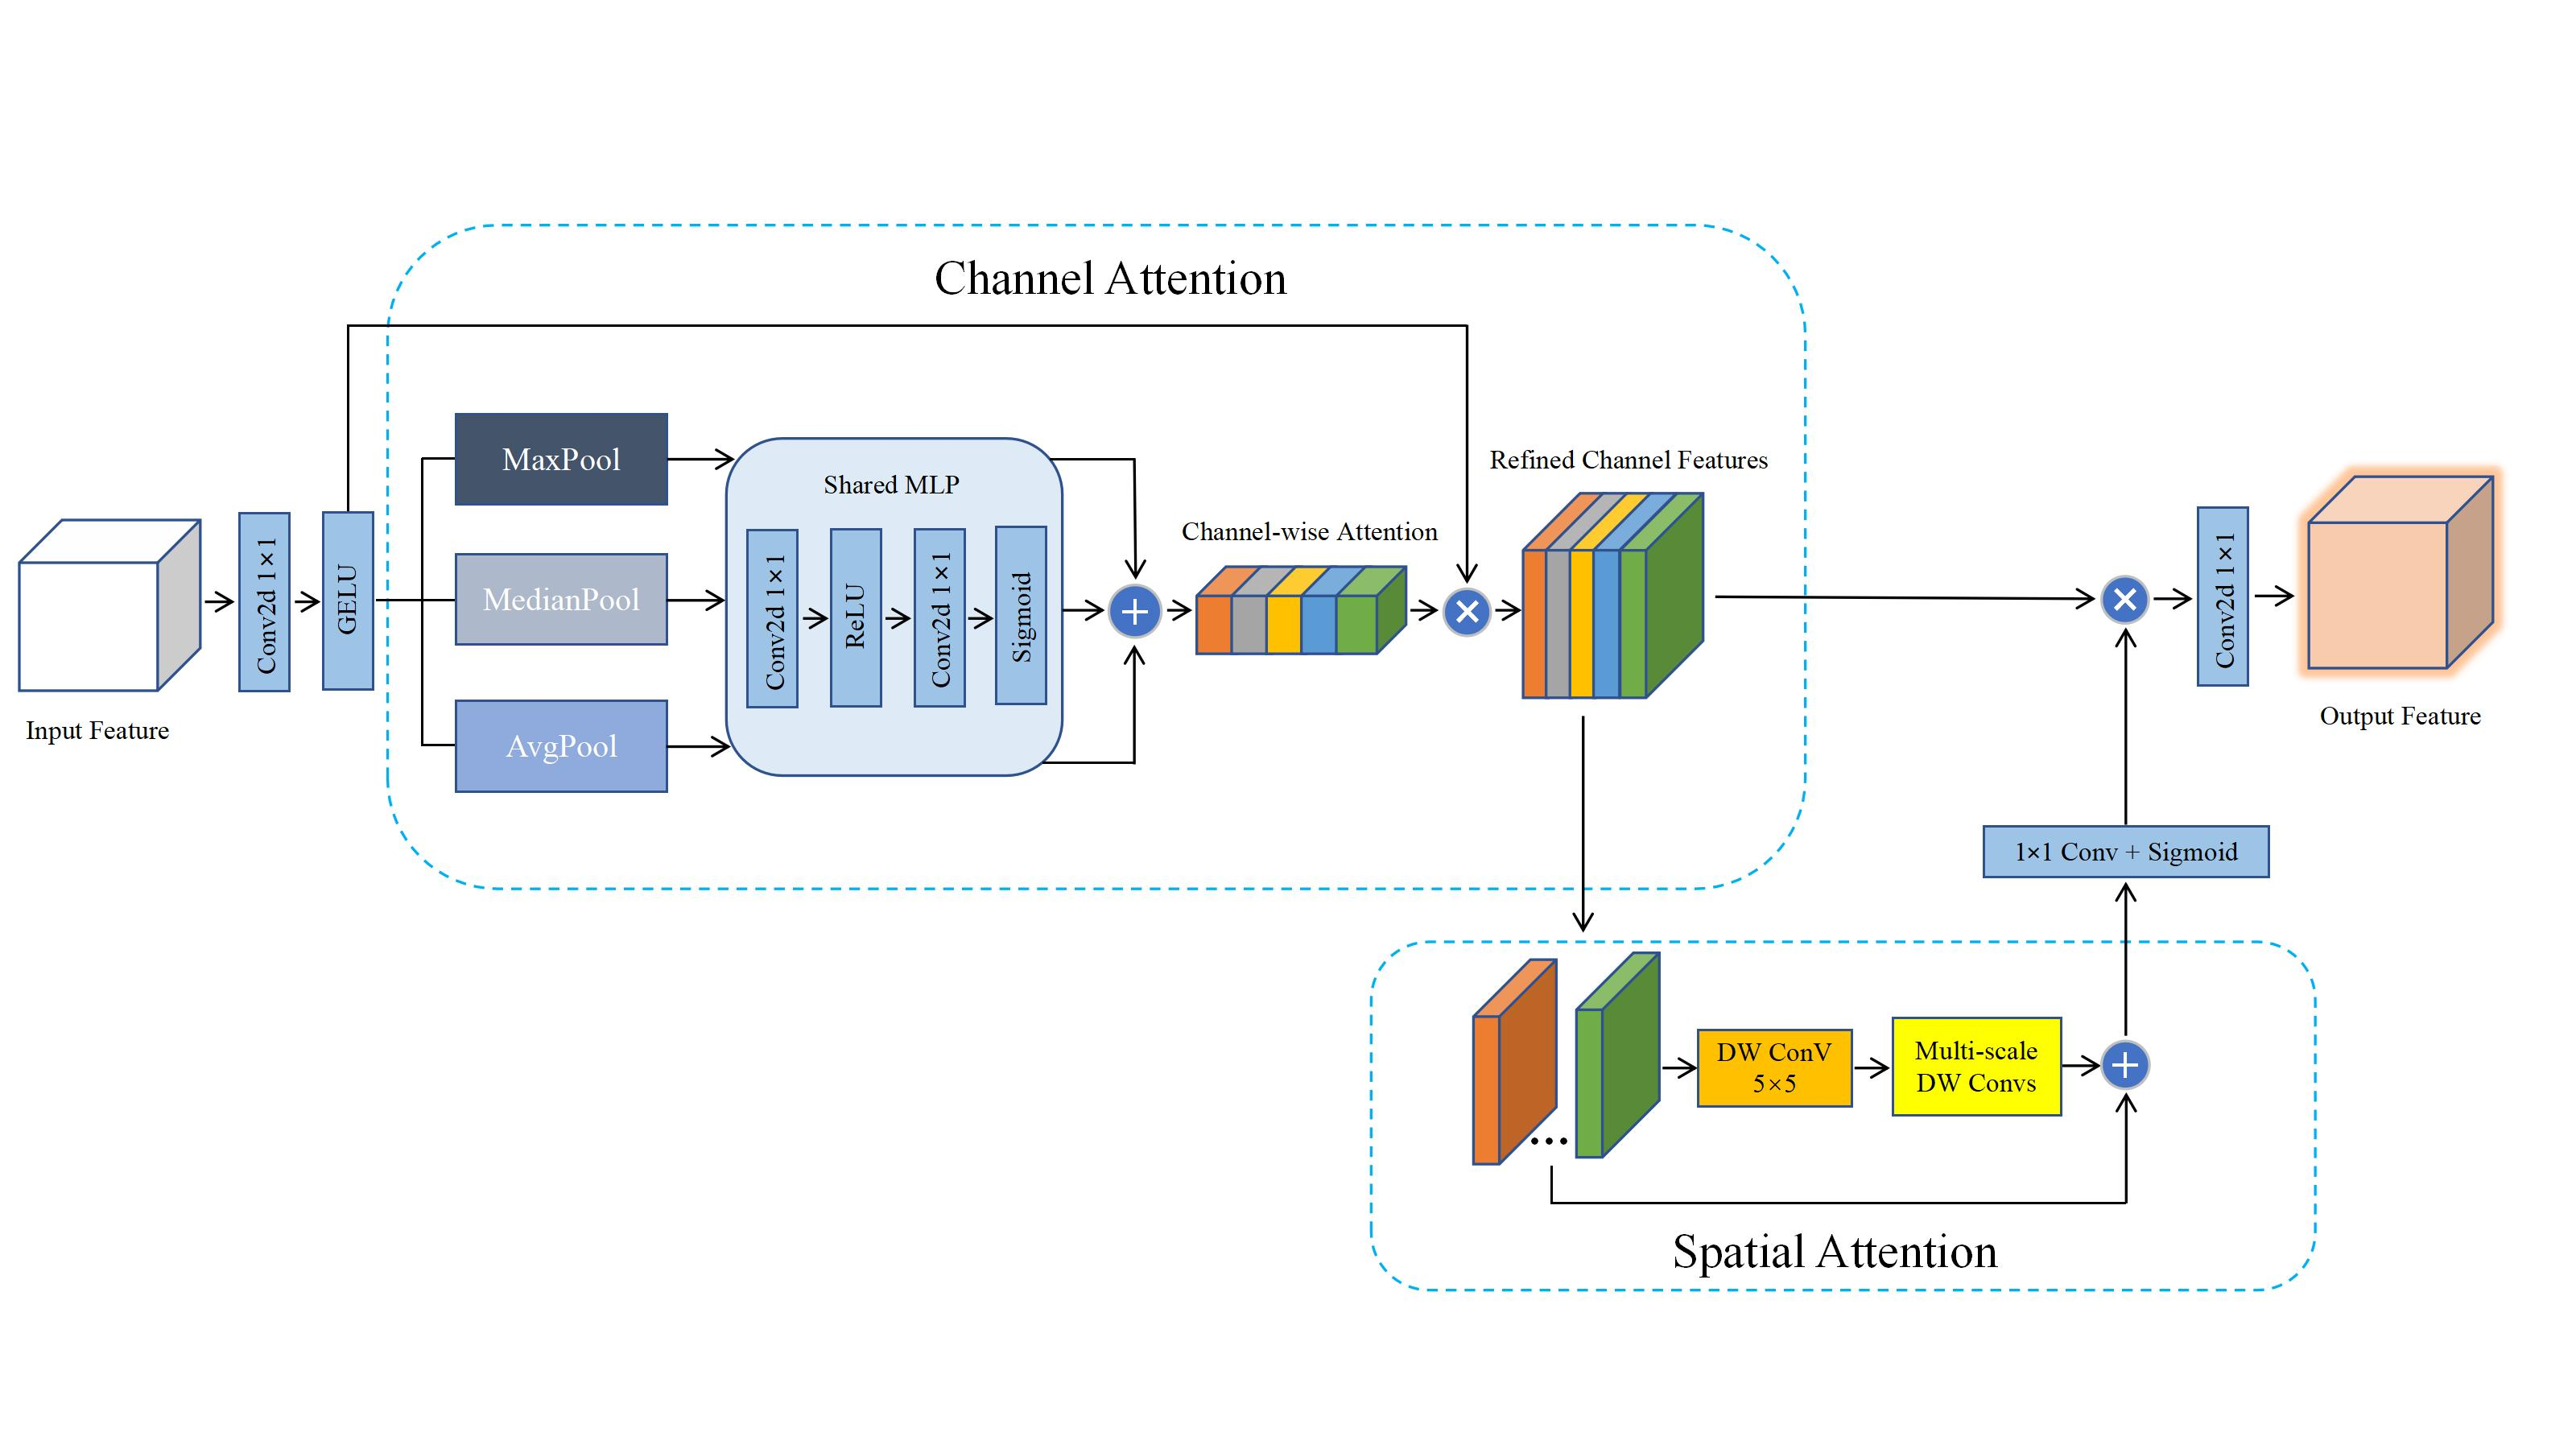
\includegraphics[width=3.3in]{模块图_01.jpg}
    \caption{\centering Illustration of the Median-enhanced Spatial and Channel Attention (MESC) module.}
    \label{figurelabel1}
\end{figure}

\subsubsection{Spatial Attention: Multi-scale Modeling for Lesion Structure}

Lesions in medical images typically exhibit significant scale variations, and discriminative features in different tasks often coexist at both local and global levels. This cross-scale feature distribution makes it difficult for convolution operations relying solely on a single receptive field to fully model key discriminative information. To address this issue, we adopt a multi-scale depthwise convolution structure:

\begin{equation}
\begin{aligned}
    F_s = \sum_{i} D_i(F_0)
\end{aligned}
\end{equation}
where \(F_0\) denotes the input feature map, and \(D_i(\cdot)\) represents depthwise convolution with different kernel sizes (i.e., different receptive fields). \(F_s\) denotes the aggregated multi-scale feature.

Based on this, we generate spatial attention maps and reweight the features:

\begin{equation}
\begin{aligned}
    F'' = A_s \odot F_s
\end{aligned}
\end{equation}
where \(A_s\) denotes the spatial attention map, and \(\odot\) represents element-wise multiplication. \(F''\) is the refined feature after spatial reweighting.

Thereby achieving self-adaptive enhancement of key lesion regions, enabling the model to more accurately focus on diagnostically significant structural regions.

\begin{figure}[thpb]
    \centering
    \includegraphics[width=3.3in]{image.png}
    \caption{\centering Illustration of the Distance-Aware Soft Target (DAST) loss.}
    \label{figurelabel2}
\end{figure}

\subsection{Distance-Aware Soft Target Loss}

Medical grading tasks typically have a well-defined ordered structure, accompanied by non-negligible annotation uncertainty. Traditional cross-entropy loss treats each category as independent and fails to capture this structure.

To address this, as depicted in the computational workflow in Fig.~\ref{figurelabel2}, we construct a soft label distribution based on category distance:

\begin{equation}
\begin{aligned}
    \tilde{y}_k = \frac{\exp\left(-\frac{|k - y|}{\tau}\right)}{\sum_{j} \exp\left(-\frac{|j - y|}{\tau}\right)}
\end{aligned}
\end{equation}
where \(y\) is the ground-truth label, \(k\) and \(j\) index class categories, and \(\tau\) is a temperature parameter controlling the smoothness of the distribution. \(\tilde{y}_k\) denotes the soft label assigned to class \(k\).

On this basis, we define the final loss:

\begin{equation}
\begin{aligned}
    \mathcal{L} = - \sum_{k} (1 - p_k)^{\gamma} \tilde{y}_k \log p_k
\end{aligned}
\end{equation}
where \(p_k\) denotes the predicted probability for class \(k\), and \(\gamma\) is the focusing parameter that emphasizes hard samples.

This loss explicitly models inter-class distance, enabling the model to tolerate ambiguity between adjacent classes while penalizing large misclassifications, thus improving robustness and generalization in medical grading tasks.

\section{Experiment}
\subsection{Datasets and Evaluation Metrics}
\subsubsection{Datasets}
\begin{table*}[!t]
    \centering
    \caption{Comparison between MESC \& DAST and classification model baseline.}
    \label{tab:performance_comparison}
    \resizebox{0.8\textwidth}{!}{
    \begin{tabular}{lcccccccc}
    \toprule
    \multirow{3}{*}{Method} & \multicolumn{2}{c}{Bone Disease} & \multicolumn{2}{c}{Lung Diseases} & \multicolumn{4}{c}{Brain Diseases} \\
    \cmidrule(lr){2-3} \cmidrule(lr){4-5} \cmidrule(lr){6-9}
    & \multicolumn{2}{c}{Knee Osteoarthritis} & \multicolumn{2}{c}{Chest X-ray Image} & \multicolumn{2}{c}{ADNI} & \multicolumn{2}{c}{Brain Tumor MRI} \\
    \cmidrule(lr){2-3} \cmidrule(lr){4-5} \cmidrule(lr){6-7} \cmidrule(lr){8-9}
    & ACC & F1-score & ACC & F1-score & ACC & F1-score & ACC & F1-score \\
    \midrule
    VGG16 & 66.00 & 0.6600 & 92.22 & 0.9194 & 98.00 & 0.9801 & 90.97 & 0.8970 \\
    VGG19 & 64.00 & 0.5800 & 95.04 & 0.9504 & 97.11 & 0.9712 & 94.83 & 0.9470 \\
    Xception & - & - & 86.02 & 0.8526 & 82.66 & 0.8265 & 91.79 & 0.9018 \\
    Inception-ResNetV2 & 63.00 & 0.6000 & 86.51 & 0.8653 & 89.65 & 0.8739 & 90.66 & 0.9077 \\
    InceptionV3 & - & - & 86.82 & 0.8479 & 68.59 & 0.7017 & 88.15 & 0.8760 \\
    DenseNet121 & 64.00 & 0.5900 & 84.27 & 0.8020 & 89.53 & 0.8980 & 91.57 & 0.9041 \\
    DenseNet169 & - & - & 87.23 & 0.8652 & 95.94 & 0.9594 & 92.23 & 0.9223 \\
    DenseNet201 & - & - & 86.37 & 0.8731 & 92.34 & 0.9243 & 91.74 & 0.9174 \\
    MobileNetV2 & 67.00 & 0.6700 & 86.68 & 0.8576 & 68.28 & 0.6824 & 91.73 & 0.9160 \\
    ViT & - & - & 89.82 & 0.9000 & 93.70 & 0.9210 & 84.71 & 0.8500 \\
    ResNet101 & 69.00 & 0.6500 & 95.36 & 0.9538 & 96.48 & 0.9726 & 88.02 & 0.8620 \\
    ResNet50V2 & - & - & 89.02 & 0.8890 & 60.62 & 0.6034 & 90.77 & 0.9081 \\
    ResNet50 & 66.12 & 0.6659 & 95.73 & 0.9562 & 94.45 & 0.9248 & 94.94 & 0.9482 \\
    \textbf{ResNet layer3+MESC+DAST} & \textbf{69.99} & \textbf{0.6956} & \textbf{96.51} & \textbf{0.9680} & \textbf{98.91} & \textbf{0.9816} & \textbf{95.62} & \textbf{0.9554} \\
    \bottomrule
\end{tabular}
    }
    \begin{tablenotes}
        \item Data sources: Knee Osteoarthritis ~\cite{28}, Chest X-ray Image ~\cite{29,30}, ADNI ~\cite{31,32,33,34}, Brain Tumor MRI ~\cite{35,36,37,38,39}.
    \end{tablenotes}
\end{table*}
We conduct experiments on five publicly available medical imaging datasets, covering diverse clinical scenarios, including skin lesion classification, chest X-ray disease recognition, Alzheimer’s disease classification, brain tumor MRI classification, and knee osteoarthritis (KOA) severity grading. These datasets are selected to evaluate the robustness and generalization ability of the proposed method across different imaging modalities and task types. In particular, the first four datasets correspond to standard multi-class classification problems, while the KOA dataset represents an ordinal grading task with inherent class ordering. The five datasets include HAM10000 (dermoscopic images with seven diagnostic categories), Chest X-ray Image (three classes: COVID-19, pneumonia, and normal), ADNI (Alzheimer’s disease classification), Brain Tumor MRI (four classes), and a Knee Osteoarthritis dataset annotated with KL grades 0–4. These datasets exhibit varying characteristics in terms of image modality, class distribution, and task difficulty, providing a comprehensive benchmark for evaluating model performance under heterogeneous medical conditions. To ensure fair comparison and reproducibility, we adopt a unified data partitioning strategy across all datasets. Specifically, for datasets without predefined splits, we apply stratified sampling to construct training, validation, and test sets while preserving class distributions. For datasets with official train/test splits, we follow the original partition and further derive a validation set from the training portion. In all cases, the final splits are approximately aligned to a common ratio (around $70\%/10\%/20\%$), ensuring consistent experimental settings across datasets.


\subsubsection{Evaluation Metrics}

We evaluate model performance using two standard metrics: Accuracy and F1-score. Accuracy measures the overall classification correctness, while F1-score provides a more balanced assessment by jointly considering precision and recall, making it more suitable for medical imaging tasks with class imbalance. This combination ensures both global performance evaluation and sensitivity to minority classes across all datasets.

\subsection{Comparative Evaluation with Baselines}
\subsubsection{Experimental Setup}
To evaluate the effectiveness of the proposed method, we conduct comparative experiments against a ResNet50 baseline, our full model (ResNet50 + layer3 + MESC + DAST), and several representative approaches under a unified experimental protocol. All models use ResNet50 as the backbone with input images resized to \(224 \times 224\). The proposed modules are inserted after the \textit{layer3} stage to enhance mid-to-high level feature representations. For fair comparison, all models are trained under identical settings, including the optimizer, learning rate schedule, batch size, and number of epochs. Specifically, we use the Adam optimizer with an initial learning rate of \(1\times10^{-4}\), a batch size of 32, and train for up to 60 epochs with a OneCycleLR scheduler. Early stopping with a patience of 15 epochs is applied based on validation performance to prevent overfitting and retain the best model.



\subsubsection{Result Analysis}
As shown in Table I, the proposed model achieves consistently competitive performance across four datasets covering both standard classification and ordinal grading tasks. Compared with the ResNet50 baseline, our method yields stable improvements on Chest X-ray Image, ADNI, and Brain Tumor MRI, indicating its effectiveness across different imaging modalities and classification scenarios. This performance trend is consistent with the design motivation of MESC, which enhances feature representation through robust channel recalibration and multi-scale spatial modeling, thereby improving the model’s ability to capture discriminative patterns under challenging conditions such as low contrast, structural complexity, and inter-class similarity. On the Knee Osteoarthritis dataset, the proposed method also achieves further improvement. This result is particularly meaningful because KOA grading has an inherent ordinal structure, where adjacent grades are often more ambiguous than distant ones. In this case, the distance-aware supervision introduced by DAST provides a better match to the task characteristics by explicitly modeling inter-class proximity, which helps reduce unreasonable long-distance errors and leads to more consistent grading predictions.

\subsection{Ablation experiment}
\subsubsection{Experimental Setup}

To further verify the effectiveness of each component in the proposed method, ablation experiments were conducted on five medical imaging datasets, namely Knee Osteoarthritis, HAM10000, Chest X-ray Image, ADNI, and Brain Tumor MRI, under the following four settings:
 
 \begin{enumerate}
    \item ResNet Baseline;
    \item ResNet Baseline + DAST;
    \item ResNet layer3 + MESC;
    \item ResNet layer3 + MESC + DAST.
\end{enumerate}
 
 Among them, Baseline + DAST is used to verify the role of distance-aware soft label loss in different tasks, layer3 + MESC is used to verify the enhancement effect of the mid-high level feature enhancement module on the representation ability of medical images, while the complete model is used to analyze the complementarity when the structural module and loss function are used in combination. Through this disassembly approach, it is possible to more clearly illustrate the contributions brought by the two core improvements proposed in this paper, namely MESC and DAST, respectively, and whether their combination can further improve the model performance.


\subsubsection{Result Analysis}


\begin{table*}[t]
    \centering
    \caption{Ablation experiments of MESC+DAST. Values are mean $\pm$ standard deviation over five seeds.}
    \label{tab:ablation_experiments}
    \resizebox{\textwidth}{!}{
    \begin{tabular}{lcccccccccc}
        \toprule
        \multirow{2}{*}{Method} & \multicolumn{3}{c}{Knee Osteoarthritis} & \multicolumn{2}{c}{Brain Tumor MRI} & \multicolumn{3}{c}{ADNI} & \multicolumn{2}{c}{Chest X-ray Image} \\
        \cmidrule(lr){2-4} \cmidrule(lr){5-6} \cmidrule(lr){7-9} \cmidrule(lr){10-11}
        & ACC & Macro-F1 & QWK & ACC & Macro-F1 & ACC & Macro-F1 & QWK & ACC & Macro-F1 \\
        \midrule
        ResNet Baseline & 66.12 $\pm$ 2.33 & 0.6659 $\pm$ 0.0058 & 0.8192 $\pm$ 0.0076 & 94.94 $\pm$ 0.42 & 0.9482 $\pm$ 0.0061 & 94.45 $\pm$ 0.84 & 0.9248 $\pm$ 0.0197 & 0.9357 $\pm$ 0.0121 & 95.73 $\pm$ 0.43 & 0.9562 $\pm$ 0.0045 \\
        ResNet Baseline + DAST & 67.32 $\pm$ 0.59 & 0.6716 $\pm$ 0.0130 & 0.8272 $\pm$ 0.0052 & 95.19 $\pm$ 0.17 & 0.9506 $\pm$ 0.0025 & 93.28 $\pm$ 1.66 & 0.9283 $\pm$ 0.0768 & 0.9435 $\pm$ 0.0189 & 96.12 $\pm$ 0.22 & 0.9630 $\pm$ 0.0022 \\
        ResNet layer3 + MESC & 68.84 $\pm$ 2.12 & 0.6762 $\pm$ 0.0204 & 0.8202 $\pm$ 0.0168 & 95.19 $\pm$ 0.16 & 0.9507 $\pm$ 0.0022 & 98.59 $\pm$ 0.26 & 0.9787 $\pm$ 0.0049 & 0.9835 $\pm$ 0.0038 & 96.51 $\pm$ 0.42 & 0.9679 $\pm$ 0.0044 \\
        \textbf{ResNet layer3 + MESC + DAST} & \textbf{69.99 $\pm$ 1.52} & \textbf{0.6956 $\pm$ 0.0117} & \textbf{0.8523 $\pm$ 0.0062} & \textbf{95.62 $\pm$ 0.50} & \textbf{0.9554 $\pm$ 0.0052} & \textbf{98.91 $\pm$ 0.45} & \textbf{0.9816 $\pm$ 0.0084} & \textbf{0.9903 $\pm$ 0.0087} & \textbf{96.51 $\pm$ 0.27} & \textbf{0.9680 $\pm$ 0.0028} \\
        \bottomrule
    \end{tabular}
    }
\end{table*}
As shown in Table II, both MESC and DAST consistently improve performance across datasets, while their effects are complementary. On general classification tasks, MESC mainly enhances feature representation by improving mid-to-high level semantic modeling, enabling the model to better capture discriminative patterns and suppress irrelevant background noise. This leads to more robust performance under challenging conditions such as class imbalance, low contrast, and complex image structures. In contrast, DAST primarily improves the training supervision by introducing soft label distributions, which help the model learn smoother and more flexible decision boundaries, resulting in more stable and balanced predictions across classes.

On the knee osteoarthritis grading task, the effect of DAST becomes more pronounced, as modeling inter-class relationships is crucial for handling ordinal labels with ambiguous boundaries. By explicitly encoding category proximity, DAST allows the model to better tolerate small deviations while reducing severe misclassifications. Meanwhile, MESC contributes by enhancing structural feature representation of joint regions, further supporting accurate grading. As a result, the full model achieves the best or most stable performance across all settings, demonstrating that combining feature enhancement (MESC) and supervision optimization (DAST) leads to consistent and complementary gains across different tasks.

\subsection{Grad-CAM Analysis}

To further investigate the interpretability of the proposed model, we visualize representative samples from five datasets using Grad-CAM, as shown in Fig.~\ref{fig:gradcam}. Across different datasets, the model consistently focuses on clinically relevant regions rather than background noise. For instance, in skin lesion images, high-response regions concentrate on lesion areas and boundaries; in chest X-ray images, activations align with abnormal pulmonary regions; in ADNI images, the model attends to brain regions related to disease-associated structural patterns; and in Brain Tumor MRI, responses are localized around tumor-related regions. These observations indicate that the proposed method effectively captures meaningful visual patterns across diverse imaging modalities.

For the knee osteoarthritis grading task, the activation patterns further reflect sensitivity to structural variations. The model primarily attends to key anatomical regions such as joint spaces and adjacent bone structures, and its focus shifts with disease severity, from subtle localized responses in early stages to more concentrated patterns in advanced cases. This suggests that the model not only learns discriminative features but also captures progression-related cues, providing interpretable support for its predictions.

% 请确保导言区有这两句：
% \usepackage{subcaption}
% \captionsetup[subfigure]{justification=centering}

\begin{figure}[htbp]
    \centering

    % First row
    \begin{subfigure}[b]{0.32\linewidth}
        \centering
        \includegraphics[width=\linewidth]{HAM10000_a.png}
        \vspace{0.2em}
        \includegraphics[width=\linewidth]{HAM10000_b.png}
        \caption{HAM10000}
    \end{subfigure}
    \hfill
    \begin{subfigure}[b]{0.32\linewidth}
        \centering
        \includegraphics[width=\linewidth]{Chest_X-ray_a.png}
        \vspace{0.2em}
        \includegraphics[width=\linewidth]{Chest_X-ray_b.png}
        \caption{Chest X-ray}
    \end{subfigure}
    \hfill
    \begin{subfigure}[b]{0.32\linewidth}
        \centering
        \includegraphics[width=\linewidth]{ADNI_a.png}
        \vspace{0.2em}
        \includegraphics[width=\linewidth]{ADNI_b.png}
        \caption{ADNI}
    \end{subfigure}

    \vspace{0.8em}

    % Second row
    \begin{subfigure}[b]{0.32\linewidth}
        \centering
        \includegraphics[width=\linewidth]{Brain_Tumor_a.png}
        \vspace{0.2em}
        \includegraphics[width=\linewidth]{Brain_Tumor_b.png}
        \caption{Brain Tumor MRI}
    \end{subfigure}
    \hfill
    \begin{subfigure}[b]{0.32\linewidth}
        \centering
        \includegraphics[width=\linewidth]{Knee_Osteoarthritis_1.png}
        \vspace{0.2em}
        \includegraphics[width=\linewidth]{Knee_Osteoarthritis_2.png}
        \caption{Knee (Moderate)}
    \end{subfigure}
    \hfill
        \begin{subfigure}[b]{0.32\linewidth}
        \centering
        \includegraphics[width=\linewidth]{Knee Osteoarthritis 3.png}
        \vspace{0.2em}
        \includegraphics[width=\linewidth]{Knee Osteoarthritis 4.png}
        \caption{Knee (Severe)}
    \end{subfigure}
    
    \caption{\centering Grad-CAM visualization on five representative datasets. For each example, the original image (top) and the corresponding activation map (bottom) are shown.}
    \label{fig:gradcam}
\end{figure}




   

\section{CONCLUSIONS}

This paper proposes a unified framework for medical image classification and grading to address the limitations of existing methods in complex structural representation and inter-class relationship modeling. Specifically, we introduce a Median-enhanced Spatial and Channel Attention (MESC) module, which improves the representation of key lesion regions and structural patterns by integrating multiple statistical cues with multi-scale spatial modeling. In addition, we propose a Distance-Aware Soft Target (DAST) loss, which explicitly incorporates inter-class distance information into training, enabling the model to distinguish adjacent errors from long-distance misclassifications in a more reasonable manner.
Experimental results on multiple public datasets, including HAM10000, Chest X-ray Image, ADNI, Brain Tumor MRI, and Knee Osteoarthritis, demonstrate that the proposed method consistently outperforms the ResNet50 baseline and achieves competitive performance on both general medical image classification and ordinal grading tasks. Further ablation studies verify the complementarity between MESC and DAST: the former mainly enhances mid- and high-level feature representation, while the latter primarily improves supervision signals and decision boundaries. Their combination leads to more stable and comprehensive performance gains. In particular, on the Knee Osteoarthritis dataset, where the ordinal relationship among classes is explicit, the distance-aware modeling of DAST further improves grading consistency, validating its effectiveness in medical grading scenarios.
Overall, the results suggest that, for medical image analysis, simply relying on deeper backbone networks is insufficient to fully address the challenges of complex feature modeling and structured classification. By combining an enhanced attention-based feature modeling mechanism with a distance-aware supervision strategy, the proposed framework provides a more effective solution for improving overall discriminative performance. Future work will focus on lighter module design, stronger cross-dataset generalization, and more rigorous validation in clinically realistic settings to further enhance the practical value of the proposed method.

\addtolength{\textheight}{-2cm}   % This command serves to balance the column lengths
                                  % on the last page of the document manually. It shortens
                                  % the textheight of the last page by a suitable amount.
                                  % This command does not take effect until the next page
                                  % so it should come on the page before the last. Make
                                  % sure that you do not shorten the textheight too much.

%%%%%%%%%%%%%%%%%%%%%%%%%%%%%%%%%%%%%%%%%%%%%%%%%%%%%%%%%%%%%%%%%%%%%%%%%%%%%%%%



%%%%%%%%%%%%%%%%%%%%%%%%%%%%%%%%%%%%%%%%%%%%%%%%%%%%%%%%%%%%%%%%%%%%%%%%%%%%%%%%



%%%%%%%%%%%%%%%%%%%%%%%%%%%%%%%%%%%%%%%%%%%%%%%%%%%%%%%%%%%%%%%%%%%%%%%%%%%%%%%%

\section*{ACKNOWLEDGMENT}

This work was completed at the Aberdeen Institute of Data Science and Artificial Intelligence, South China Normal University. The author sincerely thanks Associate Professor Yingshan Shen for her guidance and valuable suggestions on topic selection, method design, and paper writing. The author also acknowledges the creators and maintainers of the publicly available datasets used in this work, including HAM10000, Chest X-ray Image, ADNI, Brain Tumor MRI Dataset, and Knee Osteoarthritis Dataset with Severity Grading.



%%%%%%%%%%%%%%%%%%%%%%%%%%%%%%%%%%%%%%%%%%%%%%%%%%%%%%%%%%%%%%%%%%%%%%%%%%%%%%%%


\begin{thebibliography}{99}

\bibitem{1} B. Sistaninejhad, H. Rasi, and P. Nayeri, “A Review Paper about Deep Learning for Medical Image Analysis,” Computational and Mathematical Methods in Medicine, vol. 2023, no. 1, Jan. 2023, doi: 10.1155/2023/7091301.

\bibitem{2} M. D. Kohn, A. A. Sassoon, and N. D. Fernando, “Classifications in Brief: Kellgren-Lawrence Classification of Osteoarthritis,” Clinical Orthopaedics \& Related Research, vol. 474, no. 8, pp. 1886–1893, Aug. 2016, doi: 10.1007/s11999-016-4732-4.

\bibitem{3} P. Chen, L. Gao, X. Shi, K. Allen, and L. Yang, “Fully automatic knee osteoarthritis severity grading using deep neural networks with a novel ordinal loss,” Computerized Medical Imaging and Graphics, vol. 75, pp. 84–92, Jul. 2019, doi: 10.1016/j.compmedimag.2019.06.002.

\bibitem{4} K. He, X. Zhang, S. Ren, and J. Sun, “Deep Residual Learning for Image Recognition,” 2016 IEEE Conference on Computer Vision and Pattern Recognition (CVPR), pp. 770–778, Jun. 2016, doi: 10.1109/cvpr.2016.90.

\bibitem{5} J. Hu, L. Shen, and G. Sun, “Squeeze-and-Excitation Networks,” 2018 IEEE/CVF Conference on Computer Vision and Pattern Recognition, pp. 7132–7141, Jun. 2018, doi: 10.1109/cvpr.2018.00745.

\bibitem{6} S. Woo, J. Park, J.-Y. Lee, and I. S. Kweon, “CBAM: Convolutional Block Attention Module,” Computer Vision – ECCV 2018, pp. 3–19, 2018, doi: 10.1007/978-3-030-01234-2\_1.

\bibitem{7} B. Zhang, J. Tan, K. Cho, G. Chang, and C. M. Deniz, “Attention-based CNN for KL Grade Classification: Data from the Osteoarthritis Initiative,” 2020 IEEE 17th International Symposium on Biomedical Imaging (ISBI), pp. 731–735, Apr. 2020, doi: 10.1109/isbi45749.2020.9098456.

\bibitem{8} R. K. Jain, P. K. Sharma, S. Gaj, A. Sur, and P. Ghosh, “Knee osteoarthritis severity prediction using an attentive multi-scale deep convolutional neural network,” Multimedia Tools and Applications, vol. 83, no. 3, pp. 6925–6942, Jun. 2023, doi: 10.1007/s11042-023-15484-w.

\bibitem{9} R. Díaz and A. Marathe, “Soft Labels for Ordinal Regression,” 2019 IEEE/CVF Conference on Computer Vision and Pattern Recognition (CVPR), pp. 4733–4742, Jun. 2019, doi: 10.1109/cvpr.2019.00487.

\bibitem{10} W. Tang, Z. Yang, and Y. Song, “Disease-grading networks with ordinal regularization for medical imaging,” Neurocomputing, vol. 545, p. 126245, Aug. 2023, doi: 10.1016/j.neucom.2023.126245.

\bibitem{11} R. Müller, S. Kornblith, and G. Hinton, “When does label smoothing help?,” arXiv preprint arXiv:1906.02629, 2019.

\bibitem{12} J. Antony, K. McGuinness, N. E. O’Connor, and K. Moran, “Quantifying radiographic knee osteoarthritis severity using deep convolutional neural networks,” 2016 23rd International Conference on Pattern Recognition (ICPR), pp. 1195–1200, Dec. 2016, doi: 10.1109/icpr.2016.7899799.

\bibitem{13} C. Szegedy et al., “Going deeper with convolutions,” 2015 IEEE Conference on Computer Vision and Pattern Recognition (CVPR), pp. 1–9, Jun. 2015, doi: 10.1109/cvpr.2015.7298594.

\bibitem{14} F. Chollet, “Xception: Deep Learning with Depthwise Separable Convolutions,” 2017 IEEE Conference on Computer Vision and Pattern Recognition (CVPR), pp. 1800–1807, Jul. 2017, doi: 10.1109/cvpr.2017.195.

\bibitem{15} M. Sandler, A. Howard, M. Zhu, A. Zhmoginov, and L.-C. Chen, “MobileNetV2: Inverted Residuals and Linear Bottlenecks,” 2018 IEEE/CVF Conference on Computer Vision and Pattern Recognition, pp. 4510–4520, Jun. 2018, doi: 10.1109/cvpr.2018.00474.

\bibitem{16} X. Wang, R. Girshick, A. Gupta, and K. He, “Non-local Neural Networks,” 2018 IEEE/CVF Conference on Computer Vision and Pattern Recognition, pp. 7794–7803, Jun. 2018, doi: 10.1109/cvpr.2018.00813.

\bibitem{17} T.-Y. Lin, P. Goyal, R. Girshick, K. He, and P. Dollar, “Focal Loss for Dense Object Detection,” 2017 IEEE International Conference on Computer Vision (ICCV), pp. 2999–3007, Oct. 2017, doi: 10.1109/iccv.2017.324.

\bibitem{18} A. Tiulpin, J. Thevenot, E. Rahtu, P. Lehenkari, and S. Saarakkala, “Automatic Knee Osteoarthritis Diagnosis from Plain Radiographs: A Deep Learning-Based Approach,” Scientific Reports, vol. 8, no. 1, Jan. 2018, doi: 10.1038/s41598-018-20132-7.

\bibitem{19} A. Tiulpin and S. Saarakkala, “Automatic Grading of Individual Knee Osteoarthritis Features in Plain Radiographs Using Deep Convolutional Neural Networks,” Diagnostics, vol. 10, no. 11, p. 932, Nov. 2020, doi: 10.3390/diagnostics10110932.

\bibitem{20} S.-W. Pi, B.-D. Lee, M. S. Lee, and H. J. Lee, “Ensemble deep-learning networks for automated osteoarthritis grading in knee X-ray images,” Scientific Reports, vol. 13, no. 1, Dec. 2023, doi: 10.1038/s41598-023-50210-4.

\bibitem{21} H. Gu, K. Li, R. J. Colglazier, J. Yang, M. Lebhar, J. O’Donnell, W. A. Jiranek, R. C. Mather, R. J. French, N. Said, J. Zhang, C. Park, and M. A. Mazurowski, “Knee arthritis severity measurement using deep learning: A publicly available algorithm with a multi-institutional validation showing radiologist-level performance,” arXiv preprint arXiv:2203.08914, Mar. 2022.

\bibitem{22} Z. Wang et al., “Confidence-Driven Deep Learning Framework for Early Detection of Knee Osteoarthritis,” IEEE Transactions on Biomedical Engineering, vol. 73, no. 2, pp. 530–541, Feb. 2026, doi: 10.1109/tbme.2025.3587003.

\bibitem{23} A. Kurz et al., “Uncertainty Estimation in Medical Image Classification: Systematic Review,” JMIR Medical Informatics, vol. 10, no. 8, p. e36427, Aug. 2022, doi: 10.2196/36427.

\bibitem{24} A. Jungo et al., “On the Effect of Inter-observer Variability for a Reliable Estimation of Uncertainty of Medical Image Segmentation,” Medical Image Computing and Computer Assisted Intervention – MICCAI 2018, pp. 682–690, 2018, doi: 10.1007/978-3-030-00928-1\_77.

\bibitem{25} J. Lourenço-Silva and A. L. Oliveira, “Using Soft Labels to Model Uncertainty in Medical Image Segmentation,” Brainlesion: Glioma, Multiple Sclerosis, Stroke and Traumatic Brain Injuries, pp. 585–596, 2022, doi: 10.1007/978-3-031-09002-8\_52.

\bibitem{26} J. Zhang, Y. Zheng, and Y. Shi, “A Soft Label Method for Medical Image Segmentation with Multirater Annotations,” Computational Intelligence and Neuroscience, vol. 2023, no. 1, Jan. 2023, doi: 10.1155/2023/1883597.

\bibitem{27} F. C. Ghesu et al., “Quantifying and leveraging predictive uncertainty for medical image assessment,” Medical Image Analysis, vol. 68, p. 101855, Feb. 2021, doi: 10.1016/j.media.2020.101855.

\bibitem{28} A. S. Mohammed, A. A. Hasanaath, G. Latif, and A. Bashar, “Knee Osteoarthritis Detection and Severity Classification Using Residual Neural Networks on Preprocessed X-ray Images,” \textit{Diagnostics}, vol. 13, no. 8, p. 1380, 2023, doi: 10.3390/diagnostics13081380.

\bibitem{29} M. E. H. Chowdhury et al., “Can AI Help in Screening Viral and COVID-19 Pneumonia?,” IEEE Access, vol. 8, pp. 132665–132676, 2020, doi: 10.1109/access.2020.3010287.

\bibitem{30} G. I. Okolo, S. Katsigiannis, T. Althobaiti, and N. Ramzan, “On the Use of Deep Learning for Imaging-Based COVID-19 Detection Using Chest X-rays,” Sensors, vol. 21, no. 17, p. 5702, Aug. 2021, doi: 10.3390/s21175702.

\bibitem{31} R. Agarwal, A. S. Sathwik, D. Godavarthi, and J. V. Naga Ramesh, “Comparative Analysis of Deep Learning Models for Multiclass Alzheimer’s Disease Classification,” EAI Endorsed Transactions on Pervasive Health and Technology, vol. 9, Nov. 2023, doi: 10.4108/eetpht.9.4334.

\bibitem{32} A. Loddo, S. Buttau, and C. Di Ruberto, “Deep learning based pipelines for Alzheimer’s disease diagnosis: A comparative study and a novel deep-ensemble method,” Computers in Biology and Medicine, vol. 141, p. 105032, Feb. 2022, doi: 10.1016/j.compbiomed.2021.105032.

\bibitem{33} Y. Lyu, X. Yu, D. Zhu, and L. Zhang, “Classification of Alzheimer’s Disease via Vision Transformer,” Proceedings of the 15th International Conference on PErvasive Technologies Related to Assistive Environments, pp. 463–468, Jun. 2022, doi: 10.1145/3529190.3534754.

\bibitem{34} G. Sharma, A. Vijayvargiya, and R. Kumar, “Comparative Assessment among Different Convolutional Neural Network Architectures for Alzheimer’s Disease Detection,” 2021 IEEE 8th Uttar Pradesh Section International Conference on Electrical, Electronics and Computer Engineering (UPCON), pp. 1–6, Nov. 2021, doi: 10.1109/upcon52273.2021.9667607.

\bibitem{35} Balaji, R. Sen, and H. Kirty, “Detection and Classification of Brain Tumors Using Deep Convolutional Neural Networks,” arXiv preprint arXiv:2208.13264, 2022.

\bibitem{36} Md. A. A. Khandaker, Z. S. Raha, S. B. Iqbal, M. F. Mridha, and J. Shin, “From Images to Insights: Transforming Brain Cancer Diagnosis with Explainable AI,” 2024 27th International Conference on Computer and Information Technology (ICCIT), pp. 891–896, Dec. 2024, doi: 10.1109/iccit64611.2024.11022512.

\bibitem{37} H. Mehnatkesh, S. M. J. Jalali, A. Khosravi, and S. Nahavandi, “An intelligent driven deep residual learning framework for brain tumor classification using MRI images,” Expert Systems with Applications, vol. 213, p. 119087, Mar. 2023, doi: 10.1016/j.eswa.2022.119087.

\bibitem{38} Z. Rasheed et al., “Brain Tumor Classification from MRI Using Image Enhancement and Convolutional Neural Network Techniques,” Brain Sciences, vol. 13, no. 9, p. 1320, Sep. 2023, doi: 10.3390/brainsci13091320.

\bibitem{39} M. A. Talukder, M. M. Islam, and M. A. Uddin, “An Optimized Ensemble Deep Learning Model for Brain Tumor Classification,” arXiv preprint arXiv:2305.12844, 2024.


\end{thebibliography}




\end{document}
